\documentclass{article}
\usepackage{ctex}
\usepackage{amsmath}
\usepackage{amssymb}
\usepackage{bm}
\usepackage{graphicx}




\begin{document}
    \title{Note of Discrete Mathematics}
    \author{Yzy}
    \maketitle
    \tableofcontents
    
    \newtheorem{theorem}{Theorem}
    \section{Propositions 命题}
   
    \begin{theorem}
        A Propositions is a declarative  sentence that is either true or false, but not both. 
        命题就是陈述性的语句,只有“对”或者“错”。
    \end{theorem}
    conjunction 合取---$\wedge$ \quad
    disjunction 析取---$\vee$ \quad
    exclusive or---${\oplus}$ \\
    conditional statements---$p{\rightarrow}q:$ (等价于$\neg p \wedge q$)
    \footnote{条件语句作为一个数学概念不依赖于假设和结论之间的因果关系,而是用定义规定了它的真值!}
    \\
    if p, then q(若p,则q) 等价于 \textbf{p only if q(p仅当q)}
    \\
    converse(逆命题) of $p\rightarrow q$ : $q{\rightarrow}p$ \\
    contrapositive(逆否命题) of $p{\rightarrow}q$ : $\neg q{\rightarrow} \neg p$ 
    \footnote{逆否命题与原命题具有相同的真值!} 
    \\
    inverse(反命题) of $p{\rightarrow}q$ : $\neg p \rightarrow \neg q$ 
    \footnote{逆命题和反命题是等价的!}
    \\
    当两个propositions具有相同真值时,称为\underline{等价}(equivalent).\\
    $p{\leftrightarrow}q$(p当且仅当q)与$(p\rightarrow q)\wedge (q\rightarrow p)$ 等价\\

    \section{命题等价式Propositional Equvialent}
    \begin{itemize}
        \item 永真式(tautology 重言式): 永远为真。
        \item 矛盾式(contradiction): 永远为假。
        \item 可能式(contingency): 既不是永真式又不是矛盾式。
    \end{itemize}

    \subsection{逻辑等价式Logical Equvialent}
    逻辑等价:在所有情况下都有相同真值的两个复合命题,称为逻辑等价。
    记为: $p \equiv q$. (注意:$\equiv$并不是逻辑连接词) \\
    \textbf{德摩根律DeMorgan's Laws} :
    \begin{tabular}{c}
        \hline
        $\neg(p \wedge q) \equiv \neg p \vee \neg q$ \\
        \hline
        $\neg(p \vee q) \equiv \neg p \wedge \neg q$ \\
        \hline
    \end{tabular}
    \\
    构建复合命题的真值表时,有几个命题变元,真值表就有$\bm{2^{n}}$行。\\
    \textbf{27, 28页:表6,7,8 有用的逻辑等价式} \\
    有如下事实:若$p \equiv q$ 且 $q \equiv r$, 则 $p \equiv r$.

    \subsection{命题的可满足性 Propositional Satisfiability}
    $$
    \text{一个命题称为是:}
    \left\{
    \begin{aligned}
        \text{可满足的(satisfiable)}- &\text{如果\textbf{存在一个赋值}使其真值为真} \\
        \text{不可满足的(unsatisfiable)}-& \text{对\textbf{所有变元的真值赋值}都是假的} \\  
    \end{aligned}
    \right.
    $$
    \begin{itemize}
        \item 与非(NAND) $\vert$ ,顾名思义\quad $p \vert q \equiv \neg (p \wedge q)$
        \item 或非(NOR) $\downarrow$ ,同理 \quad $p \downarrow q \equiv \neg (p \vee q)$
    \end{itemize}
    $\{\neg \vee \wedge\}$,$\{\neg \vee\}$, $\{\neg \wedge\}$, $\{\downarrow\}$均是 功能完备集functional collection。
    \\
    $A_{1},...,A_{n}$均为合取式,则$A_{1}\vee A_{2} \vee ...\vee A_{n}$称为析取范式,合取范式反之亦然。   

    \subsection{谓词和量词 Predicates and Quantifiers}
    n个变量$x_1,x_2,\dots,x_n$的语句 表示成: $P(x_1,x_2,\dots,x_n)$.
    P(\dots)就是命题函数P在n元组$(x_1,x_2,\dots,x_n)$的真值。P也称为\textbf{n元谓词}。\\
    全称量词universal quantifiers
    数学命题断言某一性质对于变量在某一特定域内的所有值为真,这一特定域成为变量的\textbf{论域}(domain of discourse) 或 全体域(universe of discourse) 或 域(domain)
    \\
    \textbf{全称量词(universal quantifiers)}---$\forall$ (注:使用量词时必须先指定论域)\\
    $\forall x P(x)$表示$P(x)$的全称量化,“$P(x)$对x在其论域的所有值为真,”也读作:“对所有x,P(x)”。
    \\
    \textbf{存在量词(existential quantifiers)}---$\exists$ \\
    $\exists x P(x)$, “论域中存在一个个体x满足$P(x)$。” \\
    \textbf{唯一性量词(uniqueness quantifiers)}---$\exists!$ \\
    $\exists ! x P(x)$ 表示: 存在一个唯一的x使得P(x)为真。(有且只有一个) \\
    \textbf{约束论域}:变量必须满足的条件\textbf{直接放在量词的后面}\\
    如:\\
    $\forall x<0(x^{2}>0)$表示“对每一个满足x>0的实数x有$x^{2}>0$”---等价于:$\forall x(x<0\rightarrow x^{2}>0)$
    \\
    $\exists z>0(z^{2}=0)$ 等价于 $\exists z(z>0 \wedge z^{2}=0)$ \\
    由上可知,
    \begin{itemize}
        \item \textbf{全称量化的约束}和一个\textbf{条件语句的全称量化}等价:\\
        $\forall x(\text{约束条件})P(x) \equiv \forall x(\text{约束条件}\rightarrow P(x))$
        \item 存在量化的约束和一个\textbf{合取式的存在量化}等价
    \end{itemize}
    量词有\textbf{最高的优先级}(precedence) \\
    涉及\textbf{量词的逻辑等价式}:\\
    例:$\forall x(P(x)\wedge Q(x)) \equiv \forall xP(x) \wedge \forall xQ(x)$ 
    \\
    $\exists x(P(x)\vee Q(x)) \equiv \exists xP(x) \vee \exists xQ(x)$
    \begin{itemize}
        \item 全称量词对于一个\textbf{合取式}是可分配的,但对析取式则不可分配。
        \item 存在量词对于一个\textbf{析取式}是可分配的,但对合取式则不可分配。
    \end{itemize}
    \textbf{量化表达式的否定}\\
    量词否定的规则成为\textbf{量词的德摩根律}:\\
    $\neg \forall xP(x) \equiv \exists x \neg P(x)$ \\
    $\neg \exists xQ(x) \equiv \forall x \neg Q(x)$ \\
    \textbf{空量化 null quantification}---用于将量词\textbf{左移}\\
    (1.4练习46~49) 假设x在A中均不作为自由变元出现,且论域非空: \\
    全称量词:
    \begin{itemize}
        \item $(\forall xP(x)) \vee A \equiv \forall (xP(x) \vee A)$
        \item $(\forall xP(x))\wedge A \equiv \forall x(P(x)\wedge A)$
        \item $A \rightarrow \forall xP(x) \equiv \forall x(A \rightarrow P(x))$
        \item $\exists xP(x)\rightarrow A \equiv \forall x(P(x)\rightarrow A)$
    \end{itemize}
    存在量词:
    \begin{itemize}
        \item $(\exists xP(x))\vee A \equiv \exists x(P(x)\vee A)$
        \item $(\exists xP(x))\wedge A \equiv \exists x(P(x)\wedge A)$
        \item $A \rightarrow \exists xP(x) \equiv \exists x(A \rightarrow P(x))$
        \item $\forall xP(x)\rightarrow A \equiv \exists x(P(x)\rightarrow A)$
    \end{itemize}
    (以上逻辑等价式均可用分情况证明!)
    \subsection{嵌套量词Nested Quantifiers}
    嵌套量词,即一个量词出现在另一个量词的作用域内,如:$\forall x \exists y(x+y)=0$。注意,\textbf{量词范围内的一切都可以认为是一个命题函数}。
    \\
    $\forall x \exists y(x+y)=0$可以描述为$\forall xQ(x)$,其中$Q(x) \equiv \exists yP(x,y)$,$P(x,y) \equiv x+y=0$.
    \\
    \textbf{将量化当做循环} \\
    如要判定$\forall x \exists y P(x,y)$是否为真,对x的所有值循环。对每个x值,再对y值循环直到找到一个y使P(x,y)为真。
    如果对所有的x值都能找到一个(或以上)y值使P(x,y)为真,那么该表达式为真。\\
    $\exists x \forall yP(x,y), \exists x \exists yP(x,y)$同理。\\
    \textbf{量词顺序}\\
    在没有其他量词的语句中,在不改变量化式意义的前提下嵌套全称量词的顺序是可以改变的。\\
    \textbf{嵌套量词的否定}\\
    方法:通过连续地应用\textbf{量词的德摩根律}。\\
    例:
    $\neg (\forall x \exists y(xy=1)) = \exists x \neg \exists y(xy=1) = \exists x \forall y \neg(xy=1)
    = \exists x \forall y (xy \neq 1)
    $ \\
    注意,把$\neg$放量词后面时,不改变变元的论域,如:$\neg \forall x>0 \exists y<0 P(x,y) = \exists x>0 \neg \exists y<0 P(x,y)$
    \\
    \textbf{前束范式 prenex normal form,PNF}\\
    当且仅当表达形式为:$Q_1 x_1 Q_2 x_2 \dots Q_k x_k P(x_1,x_2,\dots,x_k)$,其中每个$Q_i$都是全称量词或者存在量词,并且$P(x_1,x_2,\dots,x_k)$是不含量词的谓词。
    \begin{itemize}
        \item[1.5 48] $\forall xP(x)\vee \forall xQ(x) \equiv \forall x \forall y(P(x)\vee Q(x))$
        \item[1.5 49] $\forall xP(x) \wedge \exists xQ(x) \equiv \forall x \exists y(P(x)\wedge Q(x))$
        \item[1.5 49] $\forall xP(x) \vee \exists xQ(x) \equiv \forall x \exists y(P(x)\vee Q(x))$
    \end{itemize}
    对\textbf{唯一性量词}有等价式:$\exists !xP(x) \equiv \exists x(P(x)\wedge \forall y(P(y)\rightarrow y=x)) \equiv \exists x \forall y (P(x)\leftrightarrow y=x)$

    \subsection{推理规则 Rules of Inference}
    论证(argument):一连串的命题并以结论作为最后的命题;\\
    有效性(valid):结论或论证的最后一个命题必须根据论证过程前面的命题或前提(premise)的真实性推出;\\
    一个论证是有效的\textbf{当且仅当}不可能出现所有前提为真而结论为假的情况,即它的所有前提为真蕴含着结论为真。\\
    谬误(fallacy):错误推理。\\
    如果前提均为真时结论为真,那么说这个论证形式是\textbf{有效的},也就是说这个推理规则是\textbf{可以用的}!\\
    永真式$(p\wedge (p\rightarrow q)) \rightarrow q$ 是\textbf{假言推理(modus ponens)}或分离规则(law of detachment)的推理规则的基础。它说明:\textbf{如果一个条件语句以及它的前提都为真,那么结论肯定为真!}
    \\
    \textbf{章节1.6.3 常用推理规则表}
    \begin{itemize}
        \item 化简律$(p\wedge q)\rightarrow p$
        \item 附加律$p\rightarrow (p\vee q)$
        \item 取拒式$(\neg q \wedge (p\rightarrow q))\rightarrow \neg p$
    \end{itemize}
    \textbf{消解律}
    $((p \vee q) \wedge(\neg p \vee r)) \rightarrow(q \vee r)$, 其中$(q \vee r)$称为消解式 \\
    常把假设和结论表示为子句(变量或其否定的一个析取式),再用消解律构造证明。
    \textbf{量化命题的推理规则}\\
    1.6.7---全称实例,全称引入,存在实例,存在引入\\
    1.6.8---命题和量化命题推理规则的组合使用:全称假言推理,全称取拒式

    \subsection{证明导论}
    定理theorem:一个能够被证明是真的语句。\\
    证明定理的方法:\\
    \begin{tabular}{|c|c|c|}
       \hline
       $p$ & $q$ & $value$\\
       \hline
       $T$ & $T$ & $T$\\
       $T$ & $F$ & $F$\\
       $F$ & $T$ & $T$\\
       $F$ & $F$ & $T$\\
       \hline
    \end{tabular}

    \begin{itemize}
        \item 直接证明法,利用条件语句$p\rightarrow q$ 来构造
        \item 间接证明法(反证法proof by contrapositive),利用$p\rightarrow q \equiv \neg q \rightarrow \neg p$这一事实来构造
        \item 空证明(vacuous proof) 即若前提$p$为假,则$p\rightarrow q$一定为真
        \item 平凡证明(trivial proof) 即若结论$q$为真,则$p\rightarrow q$一定为真
        \item 归谬证明法(proof by contradiction) 即找到一个矛盾式$r\wedge \neg r$使得$\neg p \rightarrow (r \wedge \neg r)$为真,则$p$为真
        \item 等价证明法 为了证明$p\leftrightarrow q$,即要证明$p\rightarrow q$和$q\rightarrow p$都是真的
        \item 反例证明法 要证明形如$\forall xP(x)$的语句为假,则只需要找到一个反例即可
        \item 分情形证明法 $[(p_1 \vee p_2 \vee \cdots \vee p_n)\rightarrow q] \leftrightarrow [(p_1\rightarrow q)\wedge (p_2\rightarrow q)\wedge \cdots \wedge (p_n\rightarrow q)]$
        \item 穷举证明法(proof by exhaustion) 通过检验相对少量的例子来证明
    \end{itemize}

    \textbf{不失一般性 without loss of generality(WLOG)}\\
    一般是为了缩短篇幅,即后面的情况可以采用同样的(或有明显改变)论证来完成证明。

    \section{基本结构:集合,函数,序列,求和与矩阵}
    \subsection{集合 Sets}
    集合是对象的一个无序聚集(collection),对象也称为元素(element)或成员(member)\\
    通常大写表示集合,小写表示集合中的元素。\quad $a \in A, a \notin A$\\
    可用集合构造器(set builder)来描述集合:$O=\{x \mid x \text{是小于10的正奇数}\}$ \\
    $O = \{x\in Z^+ \mid x \text{为奇数},x<10\}$\\
    \textbf{集合相等} \quad $\forall x (x\in a \leftrightarrow x\in B) \text{记为} (A=B)$,只要\textbf{元素相同},就算是\textbf{顺序不同}或者\textbf{元素出现次数不同}都是相等!
    \\
    空集(empty set or null set): $\varnothing \quad or \quad \{\}$ \\
    单元素集(singleton set): 只有一个元素的集合。如: $\{ \varnothing \}$,\textbf{但是它不是空集!}
    \\
    可以类比为:$\varnothing \rightarrow \text{一个空文件夹} \qquad \{\varnothing \} \rightarrow \text{一个文件夹中只有一个空文件夹}$
    \\
    子集(subsets): $A \subseteq B \text{当且仅当} \forall x(x\in A \rightarrow x\in B)$
    \\
    真子集(proper subsets) $A \subset B \quad \text{当且仅当} \forall x(x\in A \rightarrow x \in B) \wedge \exists x(x\in B \wedge x\notin A)$
    \\
    集合可以作为另一个集合的成员\\
    例子:$A=\{\varnothing, \{a\}, \{b\}, \{a,b\}\}, \quad B=\{x \mid x \text{是集合{a,b}的子集}\}$
    \textbf{注意到,这两个集合是相等的! 且}$a\notin A, \quad \{a\} \in A$ \\
    \subsubsection{集合的大小}
    令S为集合,若S中有\textbf{n个不同的元素},且n为非负整数,则S为有限集。n为S的基数(cardinality),记为$\mid S \mid$
    \\
    \textbf{幂集(power set)}, S的幂集是S所有子集的集合,记为$\mathcal{P}(A)$。若$\mid S \mid = n, 则\mid \mathcal{P}(S) \mid = 2^n$
    \\
    \subsubsection{笛卡尔积Cartesian Products}
    有序n元组(ordered n-tuple) $(a_1,a_2,\dots,a_n)$ 是以$a_1$为第一个元素...,是有序聚集!
    \\
    有序n元组是相等的当且仅当每一对对应的元素相等,即$a_i = b_i$ \\
    有序二元组称为\textbf{序偶}(ordered pair):(a,b), (c,d) \\
    \textbf{笛卡尔积} : $A\times B = \{(a,b) \mid a \in A \wedge b \in B\}$. 需要注意的是:若A,B不为空集,又或A,B不等,则$B\times A \neq A\times B$
    \\
    而且,$(A\times B)\times C \neq A \times B \times C$\\
    用$A^n=A\times A \times ,\dots, \times A$表示集合A与自身的笛卡尔积。\\
    笛卡尔积$A\times B$的一个子集R称为是从集合A到集合B的一个\textbf{关系 relation},R的元素是序偶,(第一个元素属于A,第二个元素属于B)。
    \\
    \textbf{真值集 truth set}\\
    将集合理论与谓词逻辑结合,给定谓词P,论域D,定义P的真值集为D中使P(x)为真的元素x组成的集合,记为$\{x \in D \mid P(x)\}$
    \\
    练习题:\\
    $\mid A \mid=m, \mid B \mid =n, then \mid A \times B \mid = mn$\\
    $\mid A \mid=m, \mid B \mid =n, \mid C\mid = p, then \mid A \times B \times C\mid = mnp$\\
    $\mid A \mid=m, and n is a integral number, then \mid A^n \mid = m^n $\\
    \textbf{求有限集的所有子集的方法}\\
    令$S=\left\{a_{1}, a_{2}, \cdots, a_{n}\right\}$,把S的每个子集用\textbf{长度为n的位串}表示,其中第i位为1当且仅当$a_i \in S$。
    为了产生S的所有子集,列出所有$2^n$个长度为n的位串,再按照对应位置写出子集即可!(即利用二进制编码实现)\\

    \subsection{集合运算}
    差集:$A-B = A \cap \overline{B}$\\
    对称差(symmetric difference)---$\oplus$, $A \oplus B$:属于A或属于B但不同时属于A与B的元素组成的集合。
    对称差常用公式:
    \begin{itemize}
        \item[对称差定义] $A\oplus B = (A\cup B)-(A \cap B)$
        \item[对称差定义] $A\oplus B = (A- B)\cup (B - A)$
        \item[交换律] $A \oplus B=B \oplus A$
        \item[结合律] $A \oplus(B \oplus C)=(A \oplus B) \oplus C$\quad 可由定义证得
        \item $(A \oplus B) \oplus B=A$
        \item $A \oplus A=\varnothing$
        \item $A \oplus \varnothing=A$
        \item $A \oplus U=\overline{A}$
        \item $A \oplus \overline{A}=U$
        \item 当$A\oplus B=C$时,$A\oplus C=B$
    \end{itemize}
    \textbf{模糊集fuzzy sets}
    全集U中每个元素在模糊集合S中都有一个隶属度,即在[0,1]范围内的实数。模糊集合S的表示法是列出元素及其隶属度(0除外)。
    \\
    \textbf{模糊集的补集}\quad 元素在$\overline{S}$中的隶属度等于1减去在S中的隶属度\\
    \textbf{模糊集的并集}\quad 元素在两个集合S,T中的隶属度最大值\\
    \textbf{模糊集的交集}\quad 元素在两个集合S,T中的隶属度最小值\\

    \subsection{函数 functions}
    也称:映射mapping, 或 变换 transformation. 对于$A\rightarrow B$的函数,A中元素在B中只能有一个指派。
    \subsubsection{一对一函数one-to-one或单射函数injection}
    $a, b \in A, \quad \forall a \forall b(f(a)=f(b) \rightarrow a=b)$
    \subsubsection{映上函数onto 或 满射函数surjection}
    即对B中每个元素b都是定义域A中某个元素的像!\\
    \subsubsection{一一对应 或 双射函数bijeciton}
    即,既是单射,又是满射!\\
    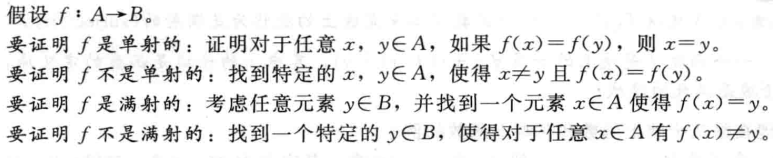
\includegraphics[width=1\textwidth]{2019-07-15_11-00.png}
    \subsubsection{反函数}
    f为A到B的一一对应。$f^{-1}$:它指派给b的元素是A中使得f(a)=b唯一的元素a。即有:当$f(a)=b$ 时 $f^{-1}(b)=a$。
    \subsubsection{函数组成}
    $(f \circ g)(a)=f(g(a))$,注意:构造函数与它的反函数不论以什么次序合成,得到的都是恒等函数!
    \subsubsection{函数的图}
    f的图为:序偶集合$\{(a,b) \mid a\in A \quad and \quad f(a)=b\}$
    \\
    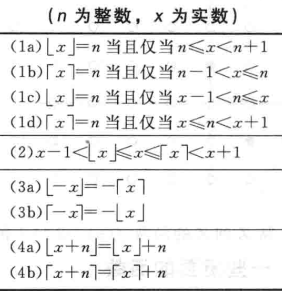
\includegraphics[width=0.8\textwidth]{2019-07-15_11-29.png}
    \subsection{序列与求和}
    \textbf{序列sequence}是一个从整数集的一个子集到一个集合S的\textbf{函数}!用记号$a_n$表示\textbf{整数n的像}。$a_n$是序列的一个项term。
    \\
    \textbf{几何级数}是这样的序列:\quad $a, ar, ,ar^2, \dots, ar^n, \dots$.\quad 可知,几何级数是指数函数$f(x)=ar^x$的离散的对应体。
    \\
    \textbf{递推关系}\\
    为序列的项找到一个显式公式,称为\textbf{闭公式closed formula},这时边说解决了带有初始条件的递推关系!
    \\
    \textbf{求和Summations}$\sum$\\
    求和式\textbf{下标平移} $\sum_{j=1}^{5}j^2 = \sum_{k=0}^{4}(k+1)^2$,\quad $\sum_{s\in \{0,2,4\}}s$表示将集合中的元素全部相加!
    \\
    \subsection{集合的基数Cardinality}
    一个有限集合(finite sets)的基数定义为该集合的元素个数。现扩展到无限(infinite sets)集合。\\
    集合A与集合B有相同的基数,当且仅当存在从A到B的一个\textbf{一一对应}。写成$|A|=|B|$。\\
    若存在一个从A到B的\textbf{一对一函数},则$|A| \leqslant|B|$。进一步,若A,B的基数不同,则$|A| < |B|$
    \subsubsection{可数集countable sets}
    把无线集分为两组,一组是与自然数集有相同的基数,另一组是具有不同基数。\\
    \textbf{正整数集,整数集,有理数集}是可数无限集。\textbf{实数集}是不可数的!
    \begin{itemize}
        \item 可数的:集合或是有限集,或与自然数集有相同的基数。记为$|S| = \aleph_0$,称作阿里夫零。
        \item 不可数的:集合不可数
    \end{itemize}
    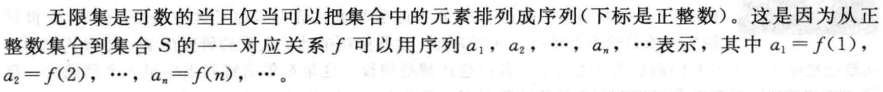
\includegraphics[width=1.20\textwidth]{2019-07-23_11-49.png}
    \begin{theorem}
        若A,B是可数集合,则$A\cup B$也是可数集合
    \end{theorem}
    \begin{theorem}
    若集合A,B存在$|A| \leqslant|B|$和$|B| \leqslant|A|$,那么$|A|=|B|$
    \end{theorem}

    \subsection{矩阵matrix}
    矩阵简便记法$\boldsymbol{A}=\left[a_{i j}\right]$, 表示A是其第(i,j)元素为$a_{ij}$的矩阵。\\
    \textbf{0-1矩阵}\\
    所有元素为0或1。两个0-1矩阵A,B的并:$\boldsymbol{A} \vee \boldsymbol{B}$;A,B的交:$\boldsymbol{A} \wedge \boldsymbol{B}$,\textbf{均为对应元素位置的布尔运算}!
    \\
    两个0-1矩阵的\textbf{布尔积}(Boolean product):$\boldsymbol{A} \odot \boldsymbol{B}$, 类似矩阵的普通乘积,但是要\textbf{用$\vee$代替加法},\textbf{用$\wedge$代替乘法}。
    \\
    0-1矩阵A的r次布尔幂记作:$\boldsymbol{A}^{[r]}$, 且$\underbrace{\boldsymbol{A}^{[r]}=\boldsymbol{A} \odot \boldsymbol{A} \odot \boldsymbol{A} \odot \cdots \odot \boldsymbol{A}}_{r\text{个}\bm{A}}$。
    \\
    另外定义$A^{[0]} \text{为} I_{n}$。

    \section{算法Algorithm}
    \subsection{algorithm}
    定义:算法是进行一项计算或解决一个问题的准确指令的有限序列。
    \subsection{函数的增长The Growth of Functions}
    


\end{document}